\section{Introduction} \label{ref:Intro}
Rare diseases affect approximately 1 in 10 Americans, constituting a significant healthcare challenge despite their individual scarcity \cite{VTNews2025_general_fact}. Accurate diagnosis remains difficult due to the vast diversity and sparsity of these conditions \cite{auvin2018problem_rarity}. While efforts to map \rev{international classification of diseases (ICD)} codes to more granular Orphanet codes have been attempted \cite{cavero2020icd10_to_orpha}, over 50\% of Orpha codes lack a direct mapping, resulting in the systematic under-reporting of rare diseases in ICD-annotated systems. Furthermore, only 2.2\% of HPO codes have matching ICD codes \cite{tan2024implications_icd_codes}. \rev{Existing rare disease differential diagnosis benchmarks rely directly on ICD labels without Orphanet or HPO concept annotations \cite{zhao2026agenticrarediseasediagnosis_deeprare}, potentially overstating real-world performance \cite{nguyen2026diagnostic_diff_diag_meta_analysis}. General purpose clinical NLP tools such as cTAKES \cite{wiegreffe2019clinical_ctakes} and MetaMap \cite{khin2017medical_metamap} inherit this same limitation, as they ground to ICD and UMLS terminologies, making automated documentation of rare disease conditions challenging.}
\rev{Mining clinical notes from EHRs offers a promising path forward, enabling direct mapping to HPO \cite{gargano2024mode_hpo} and Orphanet \cite{weinreich2008orphanet} without relying on ICD codes as intermediaries \cite{dong2023ontology_poor_annotations, yang2023enhancingphenotyperecognitionclinical}. However, real clinical notes are long, noisy, and filled with abbreviations and implicit clinical reasoning, exposing three critical gaps in existing mining approaches.}

First, existing public mining benchmarks are either poorly annotated or fail to reflect real-world clinical notes, making fine-tuning on them unreliable or infeasible. For example, our physicians found that annotations in earlier MIMIC-III rare disease mention mining attempts \cite{johnson2016mimic3, dong2023ontology_poor_annotations} frequently misinterpreted clinical abbreviations, such as interpreting NPH as normal pressure hydrocephalus'' rather than neutral protamine hagedorn'' in insulin treatment contexts. Additionally, phenotype mining approaches like RAG-HPO \cite{garcia2024_HPORAG} and PhenoGPT \cite{yang2023enhancingphenotyperecognitionclinical} evaluate on clinical case studies that lack the abbreviations and misspellings found in real clinical notes, and these case studies \cite{martinez2022raredis, yang2023enhancingphenotyperecognitionclinical} typically contain only several hundred words, whereas real clinical notes span thousands \cite{edin2023automated_medical_coding_survey, johnson2023mimic4_note}. Several studies \cite{wu2024hybrid, chen2024rarebenchllmsserverare} further rely on private annotations, impeding reproducible development. \rev{As a key consequence, approaches trained on one benchmark often fail to generalize across benchmarks with different data characteristics, and fine-tuning for specific deployment settings is frequently unrealistic, demanding methods that are robust without any task-specific training.}

Second, a substantial portion of clinically relevant phenotypes remain implicit rather than explicitly stated in notes. \rev{Identifying these requires interpreting laboratory results and applying clinical reasoning, tasks that go beyond simple entity extraction.} Conventional approaches typically follow a two-stage extract-and-match pipeline that fails to capture these implied phenotypes. Most existing methods \cite{garcia2024_HPORAG, wu2024hybrid, chen2024rarebenchllmsserverare} first extract entities and then match or verify them against ontologies like HPO \cite{gargano2024mode_hpo} or Orphanet \cite{weinreich2008orphanet} using retrieval-augmented generation (RAG) \cite{gao2024retrievalaugmentedgenerationlargelanguage_RAG_SURVEY}. Dictionary-based approaches \cite{deisseroth2019clinphen, liu2019doc2hpo, yadav2018survey_ner} like FastHPOCR \cite{groza2024fasthpocr}, while extremely efficient, lack the ability to reason about implied entities or the broader context surrounding identified mentions.

Third, privacy concerns present significant barriers to deploying capable models in practice. While cloud services increasingly adopt HIPAA compliance measures \cite{ayad2011addressing_hipaa_azure, keshetti2025designing_cloud_hipaa}, deploying LLM APIs with protected health information (PHI) typically requires extensive institutional review board (IRB) scrutiny \cite{grady2015institutional}. Locally-deployable solutions offer advantages in privacy protection and audit transparency \cite{sun2024activeprivacyauditingsupervised_whitebox_auditing}, but local deployment has historically required large, expensive hardware.

\rev{These three challenges together define what an effective mining solution must provide: generalization across data characteristics without task-specific training, reasoning capabilities that go beyond surface-level extraction, and practical deployability under real-world privacy constraints. Large language models (LLMs) have emerged as natural candidates given their flexibility, strong performance across clinical tasks \cite{wang2024surveylargelanguagemodels_biomed}, and ability to leverage existing knowledge bases such as HPO and Orphanet without extensive retraining \cite{garcia2024_HPORAG, sanmartin2024kg_rag, gao2024retrievalaugmentedgenerationlargelanguage_RAG_SURVEY}. LLMs can also provide interpretability through explanations \cite{savage2024diagnostic_interpretability}, making them well-suited for mining new phenotypes that require reasoning beyond semantic similarity. However, existing LLM-based approaches do not resolve the three challenges above: they are evaluated on private benchmarks \cite{wu2024hybrid, chen2024rarebenchllmsserverare}, rely on explicit entity extraction without reasoning about implied phenotypes \cite{garcia2024_HPORAG, wu2024hybrid}, and typically require cloud deployment of large models \cite{garcia2024_HPORAG}. Critically, we find that simply scaling to larger LLMs does not overcome these reasoning limitations, making the design of the agentic workflow, rather than model size, the determining factor in robust performance.}

\rev{To address these challenges, we propose Rare Disease Mining Agents (RDMA), an agentic framework that coordinates LLM-based reasoning across structured ontology access, implicit phenotype inference, and uncertainty-flagging for human review (Fig.~\ref{fig:RDMAvRAG}). RDMA makes three key contributions: (1) it generalizes substantially better across benchmarks without any task-specific training, outperforming fine-tuned and RAG-based baselines across datasets with different data characteristics; (2) it achieves maximal performance with a small 4-bit quantized model, reducing inference costs by up to 10x and local hardware costs by up to 17x, making private deployment on standard consumer hardware (RTX 3090) practical; and (3) its uncertainty-flagging mechanism reduces expert annotation burden while preserving agreement quality, offering a blueprint for human-AI collaboration in refining noisy clinical datasets. We hope our exploration serves as a useful guide for building rigorous rare disease benchmarks and differential diagnosis frameworks.}

\begin{figure}[htbp]
    \centering
    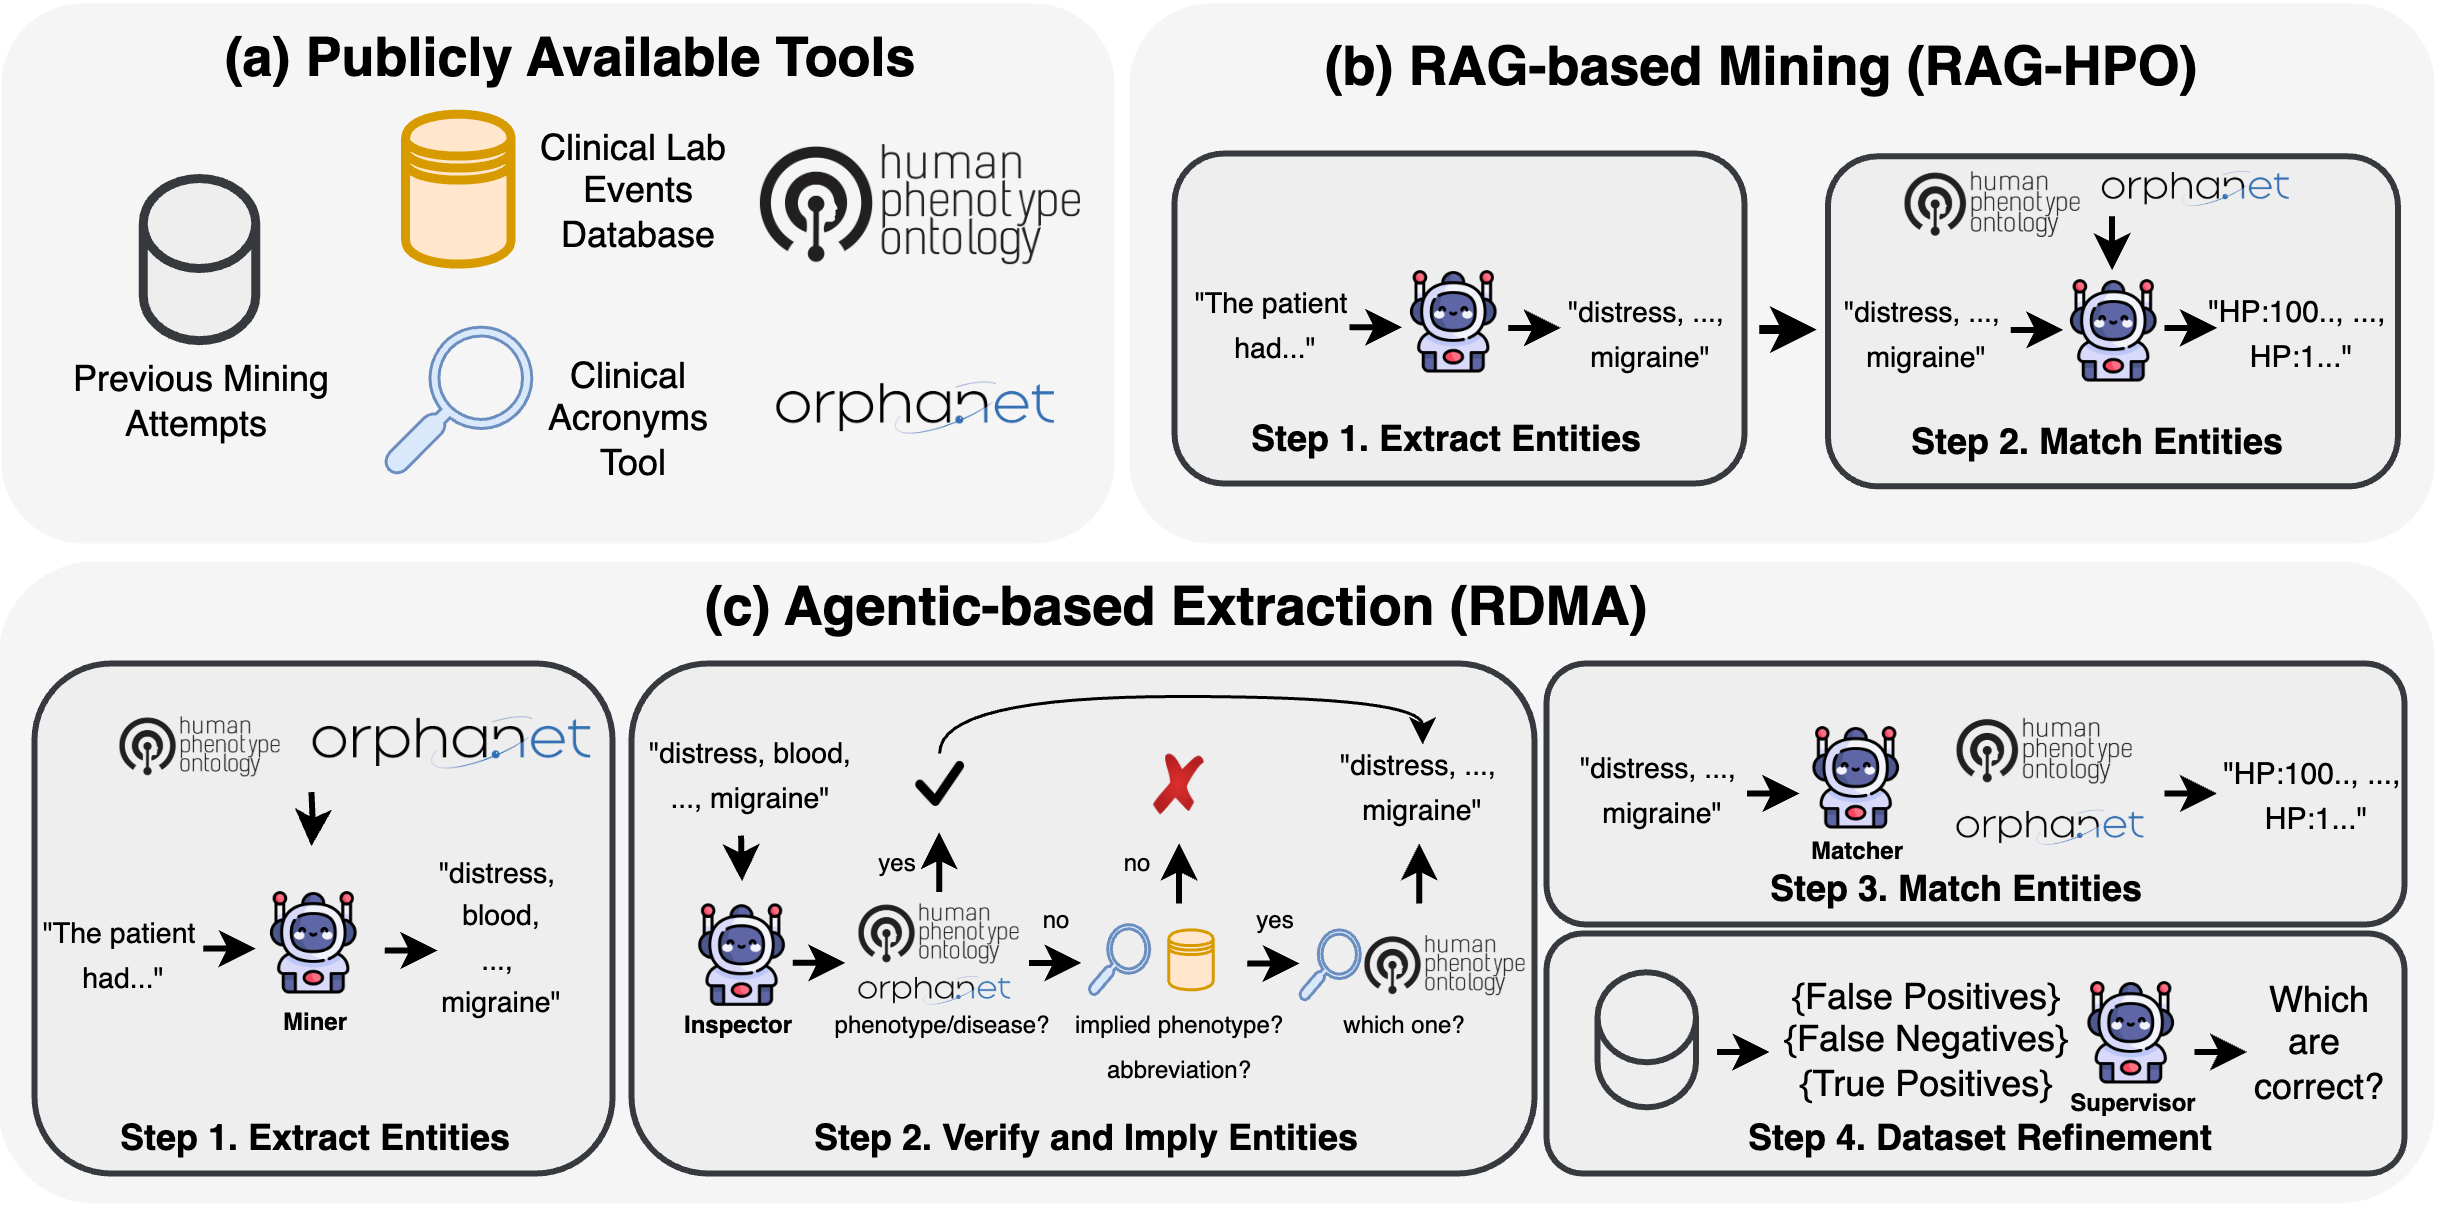
\includegraphics[width=1.0\textwidth]{figs/RDAgentVRAGHPOWithOutHuman_v2.drawio.png}
    \caption{}
    \label{fig:RDMAvRAG}
\end{figure}